\begin{figure}[h!]
	\centering
	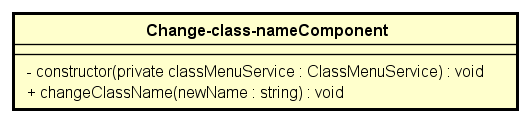
\includegraphics[scale=0.8]{res/sections/SpecificaFrontEnd/Components/Disegnetti/change-class-name.png}
	\caption{Diagramma della classe Change-class-name}
\end{figure}

\begin{itemize}
	\item \textbf{Descrizione:}\\
	Gestisce il cambiamento del nome della shape selezionata.
	\item \textbf{Utilizzo:}\\
	Viene utilizzata da EditClassMenuComponent per gestire la rinominazione delle shapes.
	\item \textbf{Metodi:}
		\begin{itemize}
			\item \emph{-constructor(private classMenuService: ClassMenuService)}\\
    		Costruttore della classe\\
    		\textbf{Parametri:}
    		\begin{itemize}
    			\item \emph{classMenuService: ClassMenuService}\\
    			Serve per creare un istanziazione di ClassMenuService
    		\end{itemize}
    		\item \emph{+changeClassName(newName: string)}\\
    		Modifica il nome della classe\\
    		\textbf{Parametri:}
    		\begin{itemize}
    			\item \emph{newName: string}\\
    			Nome della classe
    		\end{itemize}
		\end{itemize}
\end{itemize}